\begin{table}
  \centering
  \caption{Power/Energy and execution time for various core counts and compiler optimization flags}
  \label{tab:compiler-optimizations}
  \begin{tabular}{lrrrrr}
    \toprule
    \textbf{Metric / Flags} & \textbf{-O0} & \textbf{-O1} & \textbf{-O2} & \textbf{-O3} & \textbf{-O3 (fast-math)} \\
    \midrule
    \multicolumn{6}{c}{\textbf{1 core}} \\
    power/energy-pkg (J) & 52,957.47 & 5,185.28 & 4,388.12 &  4,031.83   & \textbf{4,005.70} \\
    power/energy-ram (J) & 2,208.08  & 210.28   & 183.21   &    180.00   & \textbf{168.52}  \\
    time (s)             & 270.06    & 27.453   & 24.02    &     23.5993 & \textbf{22.054}  \\
    \midrule
    \multicolumn{6}{c}{\textbf{4 cores}} \\
    power/energy-pkg (J) & 13,379.59 & 1,564.51 & 1,417.01 & \textbf{1,386.60} & 1,414.08       \\
    power/energy-ram (J) & 508.40    & 56.72    & 50.96    &     50.37         & \textbf{49.56}  \\
    time (s)             & 66.066    & 7.4351   & 6.67     &    6.5605         & \textbf{6.478}  \\
    \midrule
    \multicolumn{6}{c}{\textbf{14 cores}} \\
    power/energy-pkg (J) & 5,056.15  & 658.46   & 606.58   & \textbf{595.29}  & 639.00         \\
    power/energy-ram (J) & 153.03    & 20.79    & 18.53    & \textbf{18.24}  & 20.10          \\
    time (s)             & 19.9344   & 2.7184   & 2.42     & \textbf{2.3807} & 2.62           \\
    \midrule
    \multicolumn{6}{c}{\textbf{28 cores}} \\
    power/energy-pkg (J) & 3,650.43  & 627.89   & 565.83   &    561.59   & \textbf{547.56} \\
    power/energy-ram (J) & 120.49    & 20.00    & 18.00    &     17.93   & \textbf{17.47}  \\
    time (s)             & 15.729    & 2.6043   & 2.36     &     2.3382  & \textbf{2.2701} \\
    \midrule
    \multicolumn{6}{c}{\textbf{32 cores}} \\
    power/energy-pkg (J) & 3,353.53  & 606.52   & 552.98   &     548.83  & \textbf{535.22} \\
    power/energy-ram (J) & 110.47    & 19.54    & 17.76    &     17.58   & \textbf{17.27}  \\
    time (s)             & 14.4472   & 2.5369   & 2.33     &     2.3015  & \textbf{2.2368} \\
    \midrule
    \multicolumn{6}{c}{\textbf{60 cores}} \\
    power/energy-pkg (J) & 2,794.03  & 698.96   & 661.76   & \textbf{659.31} & 671.51         \\
    power/energy-ram (J) & 86.80     & 25.37    & 24.11    & \textbf{24.10}  & 24.76          \\
    time (s)             & 7.5463    & 1.89955  & 1.80     &     1.79288     & \textbf{1.79288}\\
    \bottomrule
  \end{tabular}
\end{table}

% --- Chart 1: Execution Time ---
\begin{figure}[h!]
  \centering
  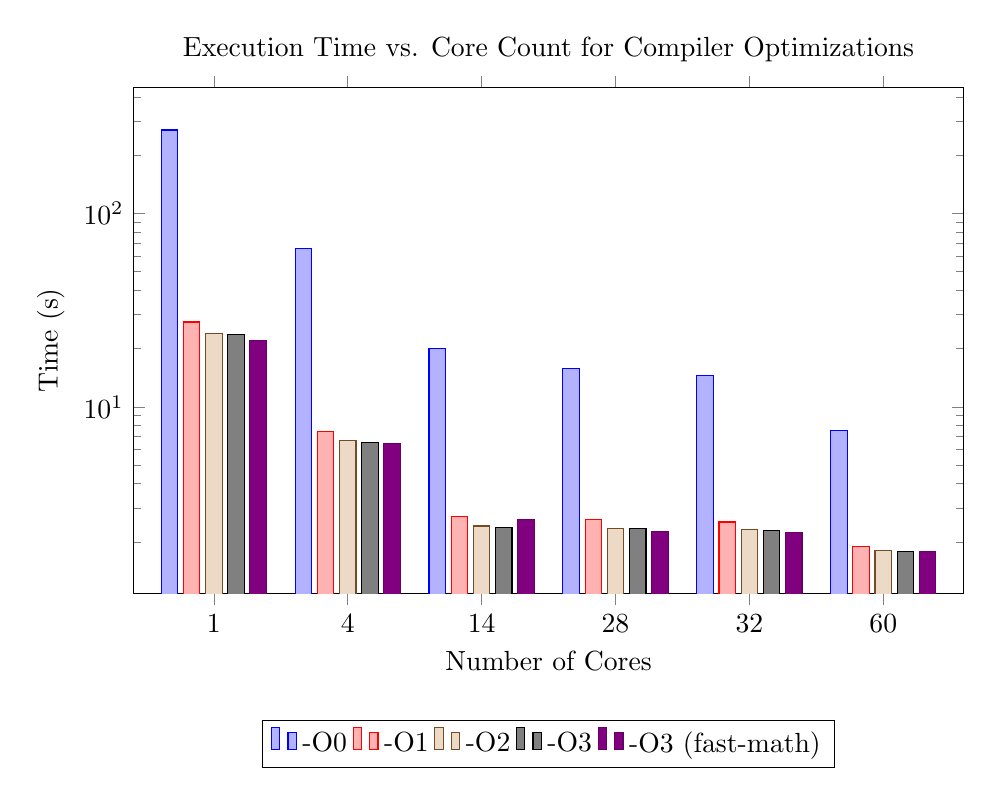
\begin{tikzpicture}
    \begin{axis}[
        title={Execution Time vs. Core Count for Compiler Optimizations},
        width=\textwidth,   % Use the full text width for the chart
        height=8cm,         % Set a fixed height for the chart
        ybar,               % This creates a vertical bar chart
        ymode=log,          % Use a logarithmic scale for the y-axis
        log basis y={10},
        enlarge x limits=0.12, % Add some space on the sides
        xlabel={Number of Cores},
        ylabel={Time (s)},
        % Define the x-axis ticks as symbolic labels
        symbolic x coords={1, 4, 14, 28, 32, 60},
        xtick=data, % Place ticks at the symbolic coordinates
        bar width=6pt, % Set the width of each individual bar
        % Position the legend below the chart
        legend style={
          at={(0.5,-0.25)},
          anchor=north,
          legend columns=-1 % Arrange legend entries horizontally
        },
        % Format the numbers on the y-axis to be readable
        yticklabel style={
            /pgf/number format/fixed,
            /pgf/number format/precision=2
        },
    ]
    % Add a plot for each optimization flag. pgfplots groups them automatically.
    \addplot coordinates {(1, 270.06) (4, 66.066) (14, 19.9344) (28, 15.729) (32, 14.4472) (60, 7.5463)};
    \addplot coordinates {(1, 27.453) (4, 7.4351) (14, 2.7184) (28, 2.6043) (32, 2.5369) (60, 1.89955)};
    \addplot coordinates {(1, 24.02) (4, 6.67) (14, 2.42) (28, 2.36) (32, 2.33) (60, 1.80)};
    \addplot coordinates {(1, 23.5993) (4, 6.5605) (14, 2.3807) (28, 2.3382) (32, 2.3015) (60, 1.79288)};
    \addplot coordinates {(1, 22.054) (4, 6.478) (14, 2.62) (28, 2.2701) (32, 2.2368) (60, 1.79288)};

    \legend{-O0, -O1, -O2, -O3, -O3 (fast-math)}
    \end{axis}
  \end{tikzpicture}
  \caption{Execution time (log scale) for various core counts and compiler flags.}
  \label{fig:time-chart}
\end{figure}

% --- Chart 2: Package Energy ---
\begin{figure}[h!]
  \centering
  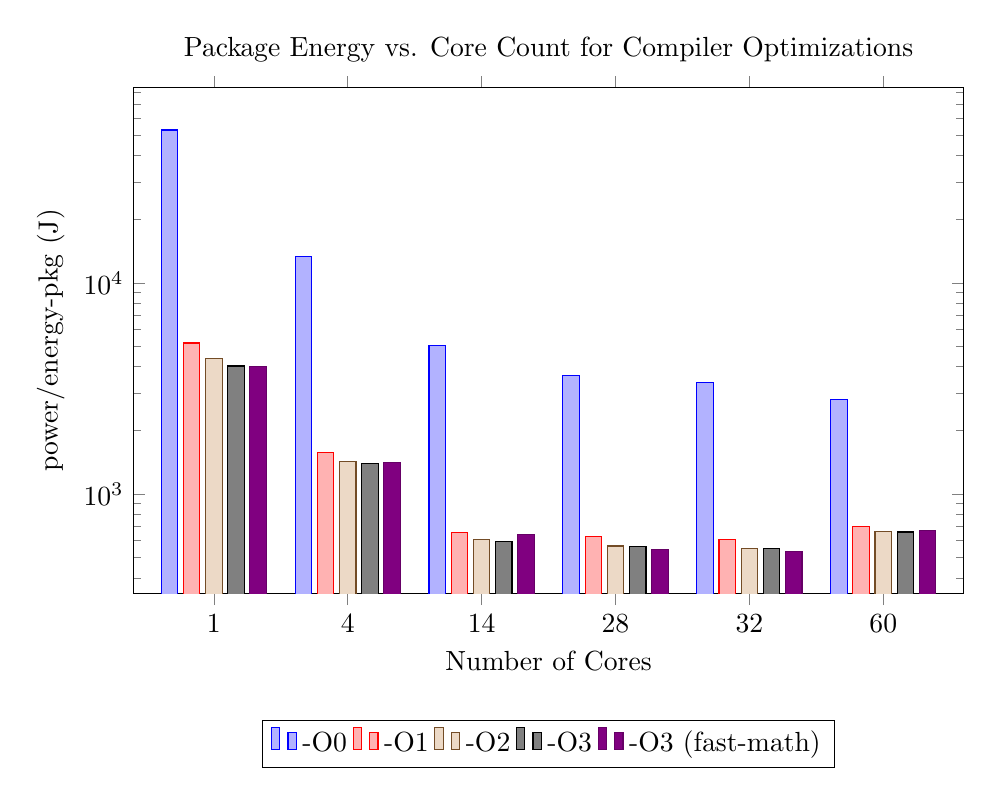
\begin{tikzpicture}
    \begin{axis}[
        title={Package Energy vs. Core Count for Compiler Optimizations},
        width=\textwidth,
        height=8cm,
        ybar,
        ymode=log,
        log basis y={10},
        enlarge x limits=0.12,
        xlabel={Number of Cores},
        ylabel={power/energy-pkg (J)},
        symbolic x coords={1, 4, 14, 28, 32, 60},
        xtick=data,
        bar width=6pt,
        legend style={
          at={(0.5,-0.25)},
          anchor=north,
          legend columns=-1
        },
        yticklabel style={
            /pgf/number format/fixed,
            /pgf/number format/precision=2
        },
    ]
    \addplot coordinates {(1, 52957.47) (4, 13379.59) (14, 5056.15) (28, 3650.43) (32, 3353.53) (60, 2794.03)};
    \addplot coordinates {(1, 5185.28) (4, 1564.51) (14, 658.46) (28, 627.89) (32, 606.52) (60, 698.96)};
    \addplot coordinates {(1, 4388.12) (4, 1417.01) (14, 606.58) (28, 565.83) (32, 552.98) (60, 661.76)};
    \addplot coordinates {(1, 4031.83) (4, 1386.60) (14, 595.29) (28, 561.59) (32, 548.83) (60, 659.31)};
    \addplot coordinates {(1, 4005.70) (4, 1414.08) (14, 639.00) (28, 547.56) (32, 535.22) (60, 671.51)};

    \legend{-O0, -O1, -O2, -O3, -O3 (fast-math)}
    \end{axis}
  \end{tikzpicture}
  \caption{Package energy consumption (log scale) for various core counts and compiler flags.}
  \label{fig:pkg-energy-chart}
\end{figure}

% --- Chart 3: RAM Energy ---
\begin{figure}[h!]
  \centering
  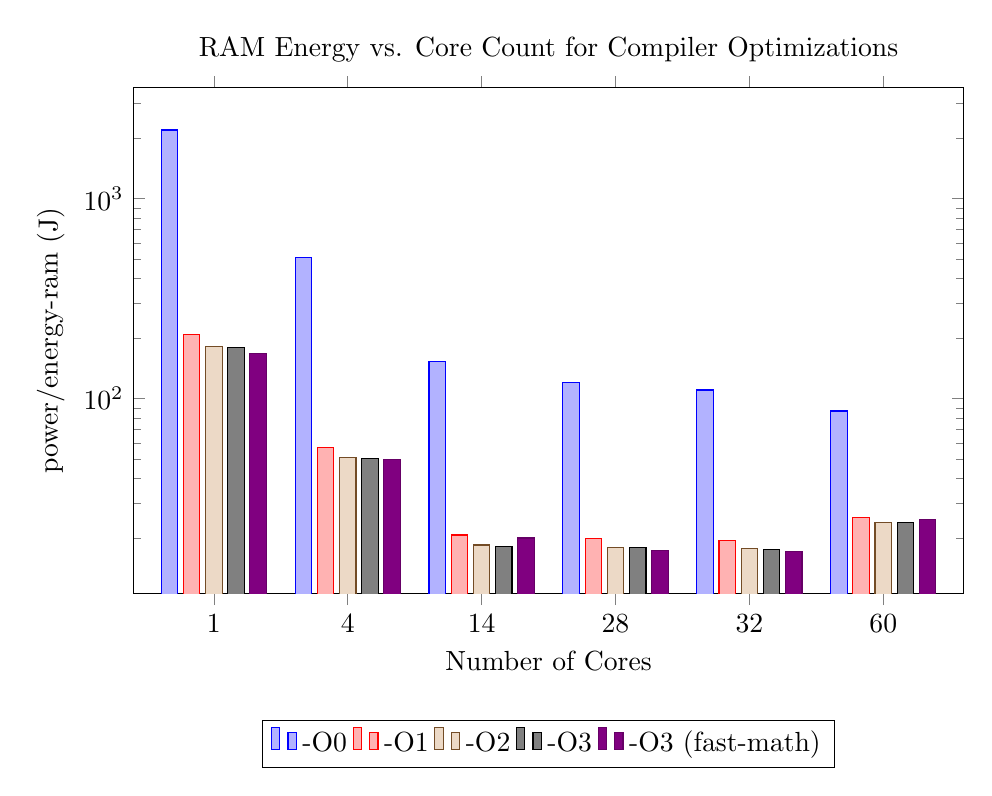
\begin{tikzpicture}
    \begin{axis}[
        title={RAM Energy vs. Core Count for Compiler Optimizations},
        width=\textwidth,
        height=8cm,
        ybar,
        ymode=log,
        log basis y={10},
        enlarge x limits=0.12,
        xlabel={Number of Cores},
        ylabel={power/energy-ram (J)},
        symbolic x coords={1, 4, 14, 28, 32, 60},
        xtick=data,
        bar width=6pt,
        legend style={
          at={(0.5,-0.25)},
          anchor=north,
          legend columns=-1
        },
        yticklabel style={
            /pgf/number format/fixed,
            /pgf/number format/precision=2
        },
    ]
    \addplot coordinates {(1, 2208.08) (4, 508.40) (14, 153.03) (28, 120.49) (32, 110.47) (60, 86.80)};
    \addplot coordinates {(1, 210.28) (4, 56.72) (14, 20.79) (28, 20.00) (32, 19.54) (60, 25.37)};
    \addplot coordinates {(1, 183.21) (4, 50.96) (14, 18.53) (28, 18.00) (32, 17.76) (60, 24.11)};
    \addplot coordinates {(1, 180.00) (4, 50.37) (14, 18.24) (28, 17.93) (32, 17.58) (60, 24.10)};
    \addplot coordinates {(1, 168.52) (4, 49.56) (14, 20.10) (28, 17.47) (32, 17.27) (60, 24.76)};

    \legend{-O0, -O1, -O2, -O3, -O3 (fast-math)}
    \end{axis}
  \end{tikzpicture}
  \caption{RAM energy consumption (log scale) for various core counts and compiler flags.}
  \label{fig:ram-energy-chart}
\end{figure}